\documentclass[dvipsnames]{beamer}
\usepackage{lmodern}
\usepackage{appendixnumberbeamer}
\renewcommand{\sfdefault}{lmss}
\renewcommand{\ttdefault}{lmtt}
\usepackage[T1]{fontenc}
% \usepackage[utf8]{inputenc}
\setcounter{secnumdepth}{3}
\setcounter{tocdepth}{3}
\usepackage{amsmath}
\usepackage{amsthm}
\usepackage{amssymb}
\theoremstyle{definition}
\newtheorem*{defn*}{\protect\definitionname}
\providecommand{\definitionname}{Definition}
\usepackage{graphicx}
\usepackage{hyperref}
\usepackage{ulem}
\PassOptionsToPackage{normalem}{ulem}
\usepackage{caption}
\usepackage{subcaption}
\usepackage{verbatim}
\usepackage[english]{babel}
\usepackage[autostyle]{csquotes}
\usepackage{tikz}
\usetikzlibrary{arrows,intersections}
\usepackage{pgfplots}
\pgfplotsset{compat = 1.15}
\usepgfplotslibrary{fillbetween}
\usepackage{verbatim}
\usepackage{booktabs}
\usepackage{multirow}
\usepackage{array}
\usepackage{nccmath}
% \usepackage{listings}
\usepackage{mathtools}

%Bibliography style, etc.
\usepackage[citestyle=authoryear-comp,natbib, uniquename = false, url = false, doi = false, uniquelist=false]{biblatex}
\renewbibmacro{in:}{}
\AtEveryBibitem{%
  \clearfield{volume}%
  \clearfield{number}
  \clearfield{month}
  \clearfield{issn}
  \clearfield{isbn}
  \clearfield{pages}
}

%\usepackage{cleveref}
\usepackage{setspace}
\makeatletter

% Macros
\providecommand{\tabularnewline}{\\}
\newcommand{\gr}{\textcolor{ForestGreen}} 
\newcommand{\rd}{\textcolor{red}}
\newcommand{\cb}{\textcolor{CornflowerBlue}} %this is the blue color you like; simply type \cb{X} where "X" is the color you want in blue
\newcommand{\vitem}{\vfill \item} %auto-centers items in lists
\newcommand{\fall}{\ \forall} %redefines "forall" (I don't like the default spacing)
\newcommand{\frall}{\quad \forall} %a \forall separated from the main math; this is the way it usually shows up in equations
\newcommand{\exist}{\ \exists} %same as \fall, but for \exists; they have the same ugly spacing
\newcommand{\R}{\mathbb{R}} %set of real numbers
\newcommand*\bigcdot{\mathpalette\bigcdot@{.5}} %different size for cdots
% \newcommand{\argmax}{\text{arg}\max}
\newenvironment{itemframe}
    {\frame{}\itemize}
    {\itemize\frame}
\newcommand\makebeamertitle{\frame{\maketitle}}%
\newtheoremstyle{named}{}{}{\itshape}{}{\bfseries}{.}{.5em}{\thmnote{#3's }#1}
\theoremstyle{named}
\newtheorem*{prop*}{Proposition}
% \newtheorem*{corollary}{Corollary}
\newtheorem*{namedtheorem}{Theorem} %allows named theorems
\newtheorem*{nameddef}{Definition}
\newtheorem{proposition}{Proposition}
\newtheorem*{assumption}{Assumption}
\newtheorem*{namedcorollary}{Corollary}
\newtheorem*{namedlemma}{Lemma}
\newtheorem*{axiom}{Axiom}
\newtheorem*{theorem*}{Theorem}
\newtheorem*{lemma*}{Lemma}
\DeclareMathOperator*{\argmin}{argmin}
\DeclareMathOperator{\argmax}{argmax}
\DeclareMathOperator{\supp}{supp}
\DeclareMathOperator{\interior}{int}
\DeclareMathOperator{\rank}{rank}
\newcolumntype{C}[1]{>{\centering\let\newline\\\arraybackslash\hspace{0pt}}m{#1}}
\newcommand{\sbt}{\,\begin{picture}(-1,1)(-1,-3)\circle*{2}\end{picture}\ }



%formatting
\usetheme{Ilmenau}
\definecolor{MIT}{rgb}{.639,.122,.204}
\definecolor{UCLA}{rgb}{0.15294117647058825, 0.4549019607843137, 0.6823529411764706}
\definecolor{UCLA_gold}{rgb}{1, 0.8196078431372549, 0}
\usecolortheme[named=UCLA]{structure}
\setbeamercolor*{palette secondary}{fg=UCLA_gold,bg=gray!15!white}
\usecolortheme{dolphin}
\setbeamertemplate{navigation symbols}{} 
\setbeamertemplate{footline}{}{}
\setbeamertemplate{headline}{}
\setbeamertemplate{navigation symbols}{}
\mode<presentation> {}
\setbeamercolor{block title}{use=structure,fg=white,bg=RoyalBlue} %blocks (theorems, etc.)in blue
\setbeamercolor{block title alerted}{use=structure,fg=white,bg=ForestGreen} %blocks (theorems, etc.)in blue

\renewcommand\qedsymbol{$\blacksquare$} %set QED symbol as black square
\renewcommand{\emph}{\textit} %set emphasized text style; this is italics
\setbeamertemplate{footline}[frame number] %slide numbers
\setbeamertemplate{itemize item}[circle] %bullet style
\setbeamertemplate{itemize subitem}{--}
\setbeamertemplate{enumerate item}[default]
\newrobustcmd*{\parentexttrack}[1]{%
  \begingroup
  \blx@blxinit
  \blx@setsfcodes
  \blx@bibopenparen#1\blx@bibcloseparen
  \endgroup}

\AtEveryCite{%
  \let\parentext=\parentexttrack%
  \let\bibopenparen=\bibopenbracket%
  \let\bibcloseparen=\bibclosebracket}

 \AtBeginDocument{%
   \let\origtableofcontents=\tableofcontents
   \def\tableofcontents{\@ifnextchar[{\origtableofcontents}{\gobbletableofcontents}}
   \def\gobbletableofcontents#1{\origtableofcontents}
 }
\newcommand{\backupbegin}{
   \newcounter{framenumberappendix}
   \setcounter{framenumberappendix}{\value{framenumber}}
}
\newcommand{\backupend}{
   \addtocounter{framenumberappendix}{-\value{framenumber}}
   \addtocounter{framenumber}{\value{framenumberappendix}} 
} 

\renewcommand{\maketitle}{
\setbeamertemplate{footline}{} 
\begin{frame}[noframenumbering]
\titlepage
\end{frame}
\setbeamertemplate{footline}[frame number]
}

\usefonttheme[onlymath]{serif}

% \usetheme{CambridgeUS}

% \newtheorem{theorem}{Theorem}
% \theoremstyle{claim}
\newtheorem{claim}{Claim}
% \newtheorem{corollary}{Corollary}


\makeatother


%\author{Drew Fudenberg}

\institute[]{}
\title{Early Life Circumstance and Adult Mental Health\\Adhvaryu, Fenske and Nyshadham, \emph{JPE} (2019)}
\author{Chris Ackerman}
\begin{document}
\maketitle

\begin{frame}{Overview}
  \begin{itemize}
  \item \textbf{Question:} How do childhood circumstances affect mental health as an adult?
    \vitem \textbf{Approach:} Diff-in-Diff, look at cocoa producing regions in Ghana.
    \vitem \textbf{Why it's special:} Mediation is really cool; can use Rodrigo's research to extend a basic diff-in-diff and get your paper published in the \emph{JPE}.
  \end{itemize}
\end{frame}
%
\begin{frame}{Setting---Mental Health}
  \begin{itemize}
  \item How does circumstance in early life affect psychological distress in adulthood?
    \vitem Depression generates losses of about 55.5 million DALYs in low- and middle-income countries.
    \vitem Use Kessler Psychological Distress Scale (K10); index of anxiety-depression mental distress
  \end{itemize}
\end{frame}
%
\begin{frame}{Setting---Cocoa in Ghana}
    \begin{figure}[htp]
      \centering
      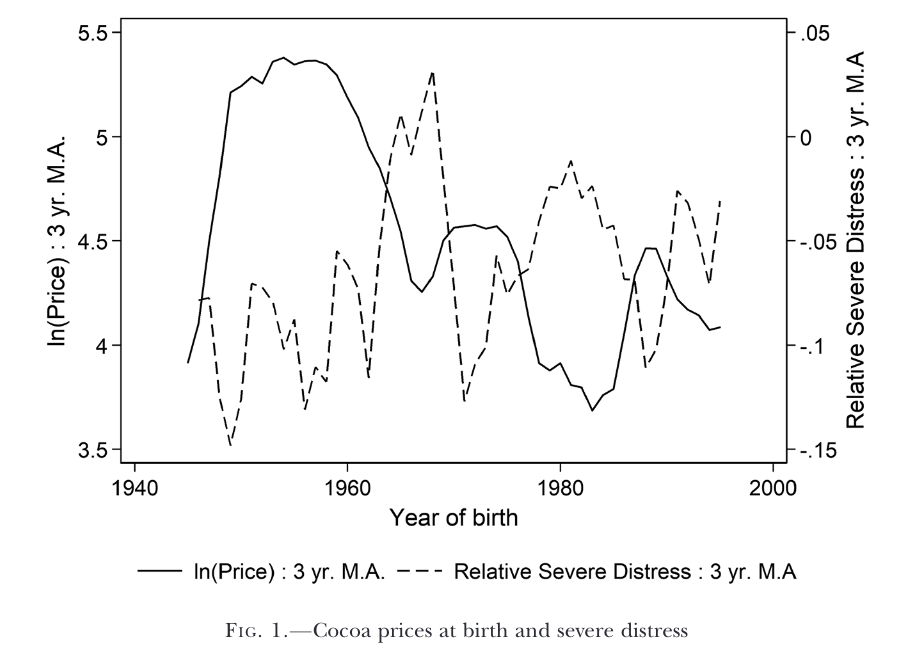
\includegraphics[width=.7\textwidth, keepaspectratio=true]{fig1.png}
    \end{figure}
  \begin{itemize}
  \item Households in the cocoa-producing regions of Ghana experience changes in the real producer price of cocoa as income shocks
    \begin{itemize}
    \item Households in regions that do not produce cocoa are unaffected
    \end{itemize}
  \end{itemize}
\end{frame}
%
\begin{frame}{Setting---Cocoa in Ghana}
    \begin{figure}[htp]
      \centering
      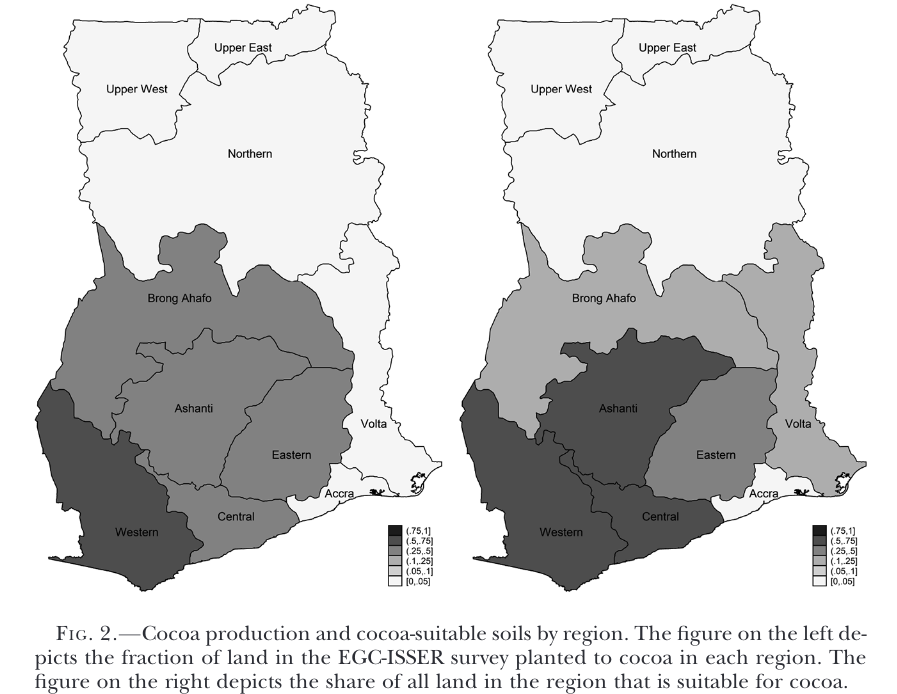
\includegraphics[width=\textwidth, keepaspectratio=true]{fig2.png}
    \end{figure}
\end{frame}
%
\begin{frame}{Setting---Cocoa in Ghana}
    \begin{figure}[htp]
      \centering
      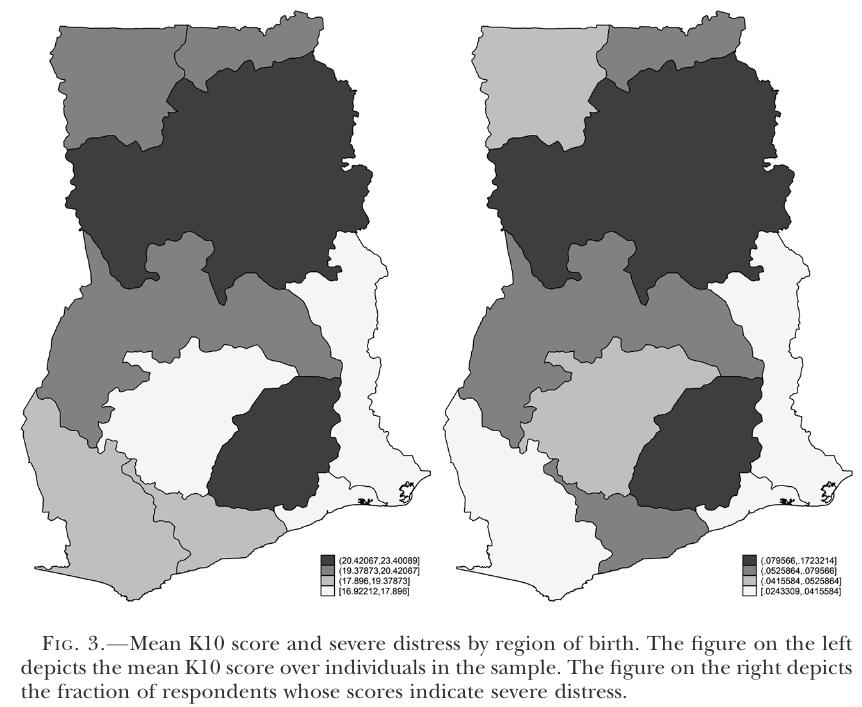
\includegraphics[width=\textwidth, keepaspectratio=true]{fig3.png}
    \end{figure}
    \end{frame}
    %
    \begin{frame}{Empirical Strategy}
      \begin{itemize}
      \item Children born to households in cocoa-growing regions during periods of high cocoa prices will have more resources
        \begin{itemize}
        \item Could have large impacts on mental health later in life
        \end{itemize}
        \vfill
        \[
\begin{aligned}
\text { Outcome }_{i r t}=& \alpha+\beta \ln \left(\text { Cocoa Price }_{t}\right) \times \text { Cocoa Producer }_{r} \\
&+x_{i r t}^{\prime} \gamma+\delta_{r}+\eta_{t}+\epsilon_{i r t}
\end{aligned}
        \]
        \vitem Outcome$_{irt}$ is the outcome for individual $i$ in region $r$, year $t$
        \begin{enumerate}
        \item Natural log of individual's response on Kessler Psychological Distress Scale
          \item Dummy for whether the score was 30 or above
        \end{enumerate}
      \end{itemize}
    \end{frame}
    %
    \begin{frame}{}
      \begin{figure}[htp]
        \centering
      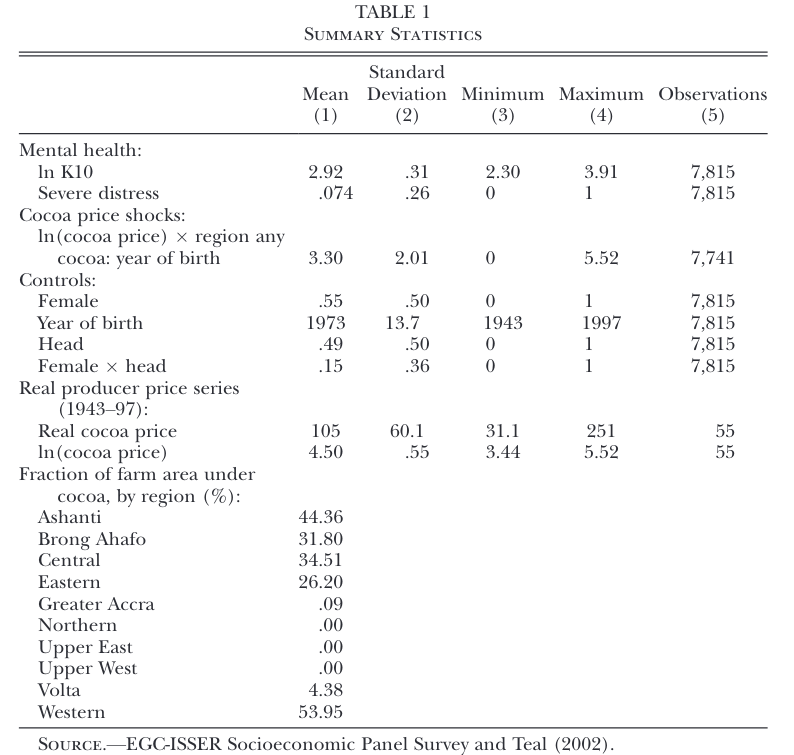
\includegraphics[height=\textheight, keepaspectratio=true]{tab1.png}  
      \end{figure}
    \end{frame}
    %
    \begin{frame}{Results (highlights)}
      \begin{itemize}
      \item Higher cocoa prices reduce mental distress; robust across specifications
        \vitem One SD price shock decreases severe mental distress by 3 percentage points (almost half the mean)
        \vitem Estimates from logit specification are about half as large as the results from the LPM
        \begin{itemize}
        \item Still statistically significant, and still large relative to baseline
        \end{itemize}
      \end{itemize}
    \end{frame}
    %
    \begin{frame}{Results---K10 Outcomes}
      \begin{figure}[htp]
        \centering
      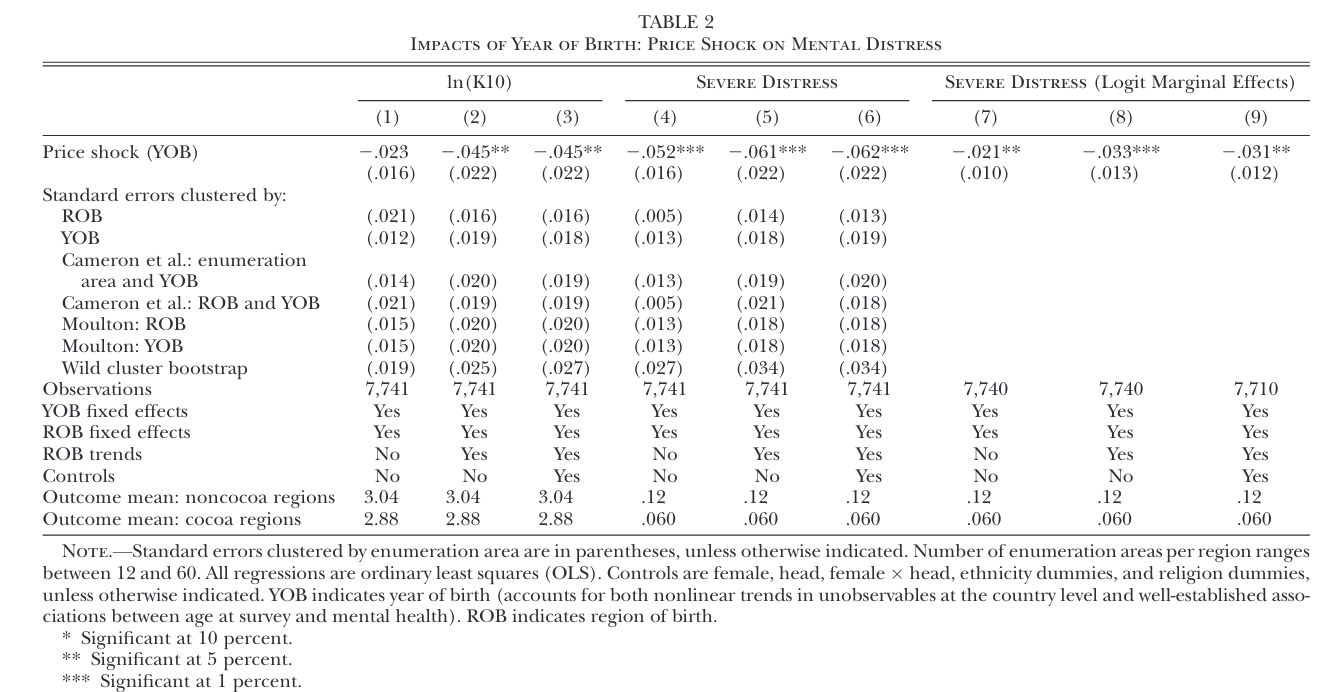
\includegraphics[width=\textwidth, keepaspectratio=true]{tab2.png}  
      \end{figure}
    \end{frame}
    %
    \begin{frame}{Mediation Analysis}
      \begin{itemize}
      \item Methodology from Heckman, Pinto, Savelyev (2013)
        \vitem Application of inverse probability weighting from Huber (2014)
        \vitem Three key assumptions:
        \begin{enumerate}
        \item Conditional independence of treatment (same as main identifying assumption)
        \item Conditional independence of mediator (may be violated; that's why they use inverse probability weighting)
          \item Common support (no mediator perfectly predicts treatment)
        \end{enumerate}
        \vitem Don't have enough data to deal with measurement error
        \vitem N.B. chose inverse probability weighting after looking at multiple approaches from Huber (2016); inverse probability weighting worked the best
      \end{itemize}
    \end{frame}
    %
    \begin{frame}{Mediation Analysis}
      Potential Mediators:
      \begin{enumerate}
      \item Cash savings
      \item Physical assets
      \item Self-employment
      \item English literacy
      \item BMI
        \item Height
        \end{enumerate}
        \begin{itemize}
          \vitem These mediators account for 10\% of the total treatment effect.
          \vitem Remaining treatment effect is either the direct effect, or mediated by something outside the data set.
        \end{itemize}
    \end{frame}
    %
    \begin{frame}{Mediation Analysis}
      \begin{figure}[htp]
        \centering
       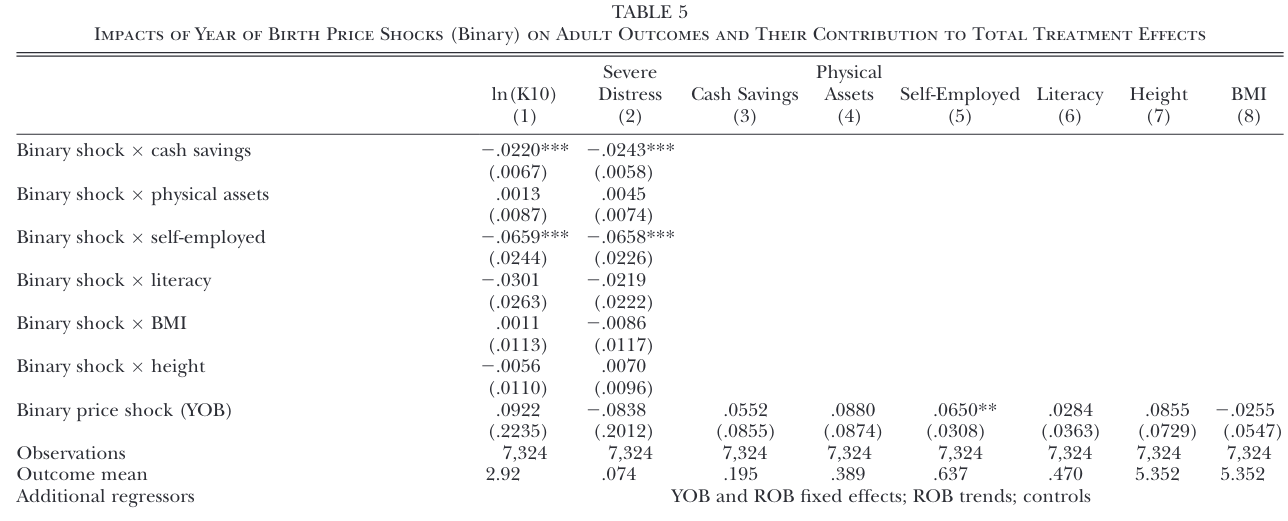
\includegraphics[width=\textwidth, keepaspectratio=true]{tab5-1.png} 
      \end{figure}
      \vspace{-3em}
      \begin{figure}[htp]
        \centering
       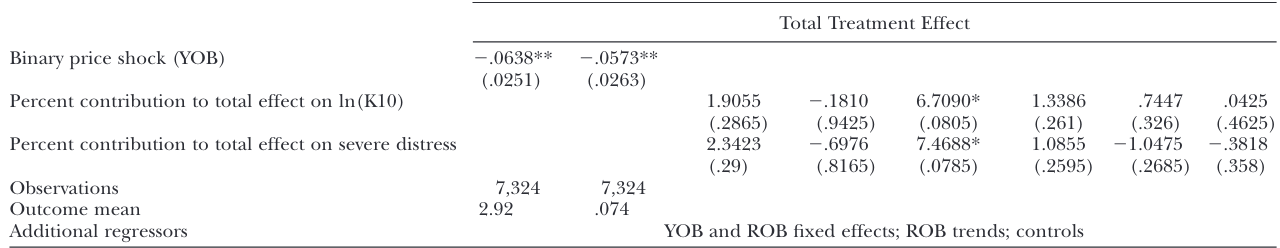
\includegraphics[width=\textwidth, keepaspectratio=true]{tab5-2.png} 
      \end{figure}
    \end{frame}
    %
    \begin{frame}
      \begin{figure}[htp]
        \centering
        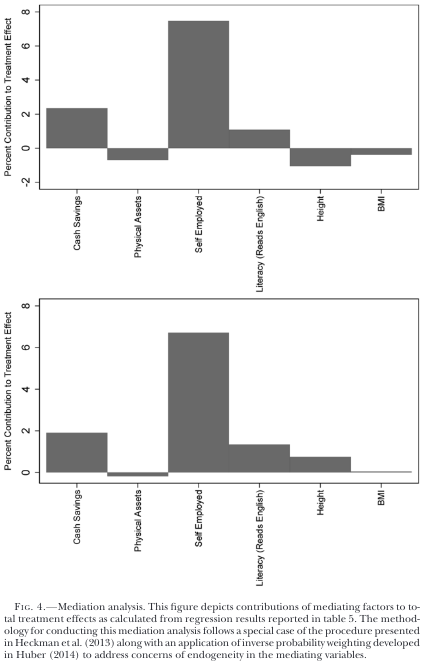
\includegraphics[height=\textheight, keepaspectratio=true]{fig4.png}
      \end{figure}
    \end{frame}
    %
    \begin{frame}{Other Mechanisms}
      \begin{itemize}
      \item Parental weight and BMI are improved by contemporaneous positive cocoa price shocks
        \vitem Positive (but imprecise) estimates for labor force participation, and substantial impacts on agricultural self-employment
        \vitem Authors interpret this as supporting evidence that impacts on mental health are coincident with improved labor, education and economic outcomes
        \vitem These estimates come from alternative datasets and \rd{cannot} be included in a proper mediation analysis
      \end{itemize}
    \end{frame}
    %
    \begin{frame}{Other Mechanisms}
      \begin{figure}[htp]
        \centering
       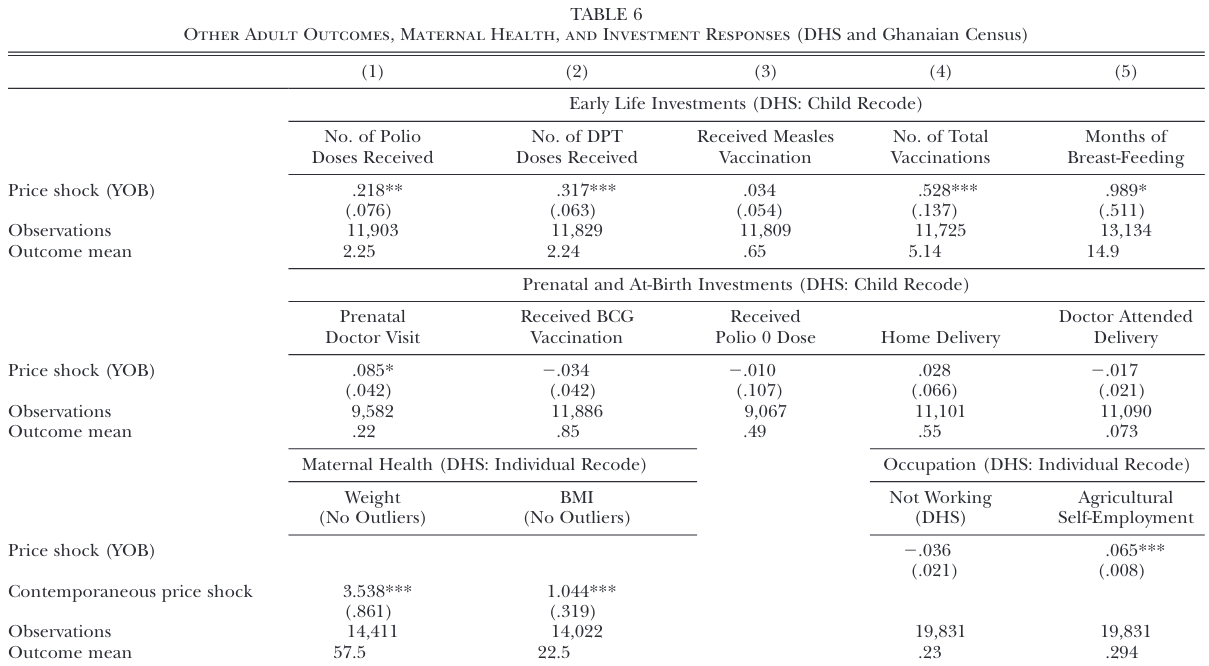
\includegraphics[width=\textwidth, keepaspectratio=true]{tab6-1.png} 
      \end{figure}
      \vspace{-1em}
      \begin{figure}[htp]
        \centering
       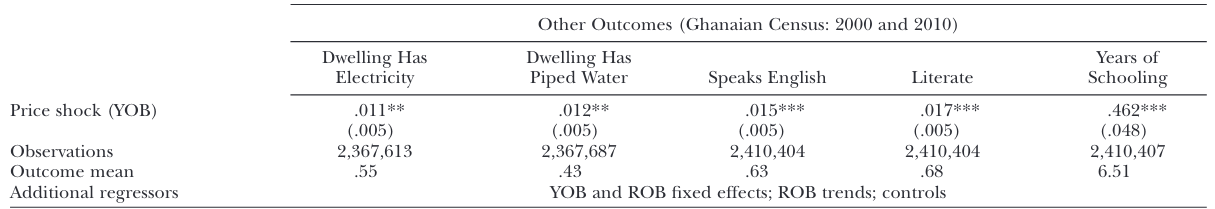
\includegraphics[width=\textwidth, keepaspectratio=true]{tab6-2.png} 
      \end{figure}
    \end{frame}
    %
    \begin{frame}{Conclusion}
      \begin{itemize}
      \item Cocoa price shocks generate income shocks for Ghanaian families
        \vitem Use diff-in-diff to see how cocoa producers benefit from this additional income
        \vitem The authors go beyond this---mediation analysis to figure out what mechanisms are accounting for the results from the diff-in-diff
        \vitem Mechanisms in the mediation analysis can only explain 10\% of the treatment effect
        \vitem Use additional data to investigate other mechanisms (but can't include these in mediation analysis)
      \end{itemize}
    \end{frame}
\end{document}
